\PassOptionsToPackage{unicode=true}{hyperref} % options for packages loaded elsewhere
\PassOptionsToPackage{hyphens}{url}
%
\documentclass[]{article}
\usepackage{lmodern}
\usepackage{amssymb,amsmath}
\usepackage{ifxetex,ifluatex}
\usepackage{fixltx2e} % provides \textsubscript
\ifnum 0\ifxetex 1\fi\ifluatex 1\fi=0 % if pdftex
  \usepackage[T1]{fontenc}
  \usepackage[utf8]{inputenc}
  \usepackage{textcomp} % provides euro and other symbols
\else % if luatex or xelatex
  \usepackage{unicode-math}
  \defaultfontfeatures{Ligatures=TeX,Scale=MatchLowercase}
\fi
% use upquote if available, for straight quotes in verbatim environments
\IfFileExists{upquote.sty}{\usepackage{upquote}}{}
% use microtype if available
\IfFileExists{microtype.sty}{%
\usepackage[]{microtype}
\UseMicrotypeSet[protrusion]{basicmath} % disable protrusion for tt fonts
}{}
\IfFileExists{parskip.sty}{%
\usepackage{parskip}
}{% else
\setlength{\parindent}{0pt}
\setlength{\parskip}{6pt plus 2pt minus 1pt}
}
\usepackage{hyperref}
\hypersetup{
            pdftitle={Practical 2: Model Evaluation},
            pdfauthor={Laura Rodriguez Navas},
            pdfborder={0 0 0},
            breaklinks=true}
\urlstyle{same}  % don't use monospace font for urls
\usepackage[margin=1in]{geometry}
\usepackage{color}
\usepackage{fancyvrb}
\newcommand{\VerbBar}{|}
\newcommand{\VERB}{\Verb[commandchars=\\\{\}]}
\DefineVerbatimEnvironment{Highlighting}{Verbatim}{commandchars=\\\{\}}
% Add ',fontsize=\small' for more characters per line
\usepackage{framed}
\definecolor{shadecolor}{RGB}{248,248,248}
\newenvironment{Shaded}{\begin{snugshade}}{\end{snugshade}}
\newcommand{\AlertTok}[1]{\textcolor[rgb]{0.94,0.16,0.16}{#1}}
\newcommand{\AnnotationTok}[1]{\textcolor[rgb]{0.56,0.35,0.01}{\textbf{\textit{#1}}}}
\newcommand{\AttributeTok}[1]{\textcolor[rgb]{0.77,0.63,0.00}{#1}}
\newcommand{\BaseNTok}[1]{\textcolor[rgb]{0.00,0.00,0.81}{#1}}
\newcommand{\BuiltInTok}[1]{#1}
\newcommand{\CharTok}[1]{\textcolor[rgb]{0.31,0.60,0.02}{#1}}
\newcommand{\CommentTok}[1]{\textcolor[rgb]{0.56,0.35,0.01}{\textit{#1}}}
\newcommand{\CommentVarTok}[1]{\textcolor[rgb]{0.56,0.35,0.01}{\textbf{\textit{#1}}}}
\newcommand{\ConstantTok}[1]{\textcolor[rgb]{0.00,0.00,0.00}{#1}}
\newcommand{\ControlFlowTok}[1]{\textcolor[rgb]{0.13,0.29,0.53}{\textbf{#1}}}
\newcommand{\DataTypeTok}[1]{\textcolor[rgb]{0.13,0.29,0.53}{#1}}
\newcommand{\DecValTok}[1]{\textcolor[rgb]{0.00,0.00,0.81}{#1}}
\newcommand{\DocumentationTok}[1]{\textcolor[rgb]{0.56,0.35,0.01}{\textbf{\textit{#1}}}}
\newcommand{\ErrorTok}[1]{\textcolor[rgb]{0.64,0.00,0.00}{\textbf{#1}}}
\newcommand{\ExtensionTok}[1]{#1}
\newcommand{\FloatTok}[1]{\textcolor[rgb]{0.00,0.00,0.81}{#1}}
\newcommand{\FunctionTok}[1]{\textcolor[rgb]{0.00,0.00,0.00}{#1}}
\newcommand{\ImportTok}[1]{#1}
\newcommand{\InformationTok}[1]{\textcolor[rgb]{0.56,0.35,0.01}{\textbf{\textit{#1}}}}
\newcommand{\KeywordTok}[1]{\textcolor[rgb]{0.13,0.29,0.53}{\textbf{#1}}}
\newcommand{\NormalTok}[1]{#1}
\newcommand{\OperatorTok}[1]{\textcolor[rgb]{0.81,0.36,0.00}{\textbf{#1}}}
\newcommand{\OtherTok}[1]{\textcolor[rgb]{0.56,0.35,0.01}{#1}}
\newcommand{\PreprocessorTok}[1]{\textcolor[rgb]{0.56,0.35,0.01}{\textit{#1}}}
\newcommand{\RegionMarkerTok}[1]{#1}
\newcommand{\SpecialCharTok}[1]{\textcolor[rgb]{0.00,0.00,0.00}{#1}}
\newcommand{\SpecialStringTok}[1]{\textcolor[rgb]{0.31,0.60,0.02}{#1}}
\newcommand{\StringTok}[1]{\textcolor[rgb]{0.31,0.60,0.02}{#1}}
\newcommand{\VariableTok}[1]{\textcolor[rgb]{0.00,0.00,0.00}{#1}}
\newcommand{\VerbatimStringTok}[1]{\textcolor[rgb]{0.31,0.60,0.02}{#1}}
\newcommand{\WarningTok}[1]{\textcolor[rgb]{0.56,0.35,0.01}{\textbf{\textit{#1}}}}
\usepackage{graphicx,grffile}
\makeatletter
\def\maxwidth{\ifdim\Gin@nat@width>\linewidth\linewidth\else\Gin@nat@width\fi}
\def\maxheight{\ifdim\Gin@nat@height>\textheight\textheight\else\Gin@nat@height\fi}
\makeatother
% Scale images if necessary, so that they will not overflow the page
% margins by default, and it is still possible to overwrite the defaults
% using explicit options in \includegraphics[width, height, ...]{}
\setkeys{Gin}{width=\maxwidth,height=\maxheight,keepaspectratio}
\setlength{\emergencystretch}{3em}  % prevent overfull lines
\providecommand{\tightlist}{%
  \setlength{\itemsep}{0pt}\setlength{\parskip}{0pt}}
\setcounter{secnumdepth}{0}
% Redefines (sub)paragraphs to behave more like sections
\ifx\paragraph\undefined\else
\let\oldparagraph\paragraph
\renewcommand{\paragraph}[1]{\oldparagraph{#1}\mbox{}}
\fi
\ifx\subparagraph\undefined\else
\let\oldsubparagraph\subparagraph
\renewcommand{\subparagraph}[1]{\oldsubparagraph{#1}\mbox{}}
\fi

% set default figure placement to htbp
\makeatletter
\def\fps@figure{htbp}
\makeatother


\title{Practical 2: Model Evaluation}
\author{Laura Rodriguez Navas}
\date{January 2020}

\begin{document}
\maketitle

\hypertarget{question-1}{%
\subsubsection{Question 1}\label{question-1}}

Load the data into R. Name the columns to better identify the board, as
visited from left to right and from top to down.

\begin{Shaded}
\begin{Highlighting}[]
\NormalTok{data <-}\StringTok{ }\KeywordTok{read.table}\NormalTok{(}\StringTok{"tic-tac-toe.data.txt"}\NormalTok{, }\DataTypeTok{header=}\OtherTok{FALSE}\NormalTok{, }\DataTypeTok{sep=}\StringTok{","}\NormalTok{)}
\KeywordTok{names}\NormalTok{(data) <-}\StringTok{ }\KeywordTok{c}\NormalTok{(}\StringTok{"top-left-square"}\NormalTok{, }
                 \StringTok{"top-middle-square"}\NormalTok{, }
                 \StringTok{"top-right-square"}\NormalTok{, }
                 \StringTok{"middle-left-square"}\NormalTok{, }
                 \StringTok{"middle-middle-square"}\NormalTok{, }
                 \StringTok{"middle-right-square"}\NormalTok{, }
                 \StringTok{"bottom-left-square"}\NormalTok{, }
                 \StringTok{"bottom-middle-square"}\NormalTok{,}
                 \StringTok{"bottom-right-square"}\NormalTok{, }
                 \StringTok{"Class"}\NormalTok{)}
\KeywordTok{str}\NormalTok{(data)}
\end{Highlighting}
\end{Shaded}

\begin{verbatim}
## 'data.frame':    958 obs. of  10 variables:
##  $ top-left-square     : Factor w/ 3 levels "b","o","x": 3 3 3 3 3 3 3 3 3 3 ...
##  $ top-middle-square   : Factor w/ 3 levels "b","o","x": 3 3 3 3 3 3 3 3 3 3 ...
##  $ top-right-square    : Factor w/ 3 levels "b","o","x": 3 3 3 3 3 3 3 3 3 3 ...
##  $ middle-left-square  : Factor w/ 3 levels "b","o","x": 3 3 3 3 3 3 3 3 3 3 ...
##  $ middle-middle-square: Factor w/ 3 levels "b","o","x": 2 2 2 2 2 2 2 2 2 1 ...
##  $ middle-right-square : Factor w/ 3 levels "b","o","x": 2 2 2 2 2 2 1 1 1 2 ...
##  $ bottom-left-square  : Factor w/ 3 levels "b","o","x": 3 2 2 2 1 1 2 2 1 2 ...
##  $ bottom-middle-square: Factor w/ 3 levels "b","o","x": 2 3 2 1 2 1 2 1 2 2 ...
##  $ bottom-right-square : Factor w/ 3 levels "b","o","x": 2 2 3 1 1 2 1 2 2 1 ...
##  $ Class               : Factor w/ 2 levels "negative","positive": 2 2 2 2 2 2 2 2 2 2 ...
\end{verbatim}

Make valid column names.

\begin{Shaded}
\begin{Highlighting}[]
\KeywordTok{colnames}\NormalTok{(data) <-}\StringTok{ }\KeywordTok{make.names}\NormalTok{(}\KeywordTok{colnames}\NormalTok{(data))}
\end{Highlighting}
\end{Shaded}

Check for missing values.

\begin{Shaded}
\begin{Highlighting}[]
\KeywordTok{any}\NormalTok{(}\KeywordTok{is.na}\NormalTok{(data))}
\end{Highlighting}
\end{Shaded}

\begin{verbatim}
## [1] FALSE
\end{verbatim}

\hypertarget{question-2}{%
\subsubsection{Question 2}\label{question-2}}

Read the ``data splitting'' section at the web page of caret. Then split
the data into 70\% training and 30\% test by keeping the original
proportion of classes.

\begin{Shaded}
\begin{Highlighting}[]
\KeywordTok{set.seed}\NormalTok{(}\DecValTok{825}\NormalTok{)}
\NormalTok{inTraining <-}\StringTok{ }\KeywordTok{createDataPartition}\NormalTok{(data}\OperatorTok{$}\NormalTok{Class, }\DataTypeTok{p=}\NormalTok{.}\DecValTok{7}\NormalTok{, }\DataTypeTok{list=}\OtherTok{FALSE}\NormalTok{)}
\NormalTok{data_training <-}\StringTok{ }\NormalTok{data[ inTraining,]}
\NormalTok{data_testing  <-}\StringTok{ }\NormalTok{data[}\OperatorTok{-}\NormalTok{inTraining,]}
\end{Highlighting}
\end{Shaded}

\hypertarget{question-3}{%
\subsubsection{Question 3}\label{question-3}}

Specifiy the type of resampling.

\begin{Shaded}
\begin{Highlighting}[]
\NormalTok{fitControl <-}\StringTok{ }\KeywordTok{trainControl}\NormalTok{(}\DataTypeTok{method=}\StringTok{"repeatedcv"}\NormalTok{, }
                           \DataTypeTok{number=}\DecValTok{10}\NormalTok{, }
                           \DataTypeTok{repeats=}\DecValTok{1}\NormalTok{,}
                           \DataTypeTok{classProbs=}\OtherTok{TRUE}\NormalTok{)}
\end{Highlighting}
\end{Shaded}

Apply the models: Naive Bayes, Decision Tree, Neural Networks, Nearest
Neighbour and SVM (linear kernel) to the data training dataset and using
the same seed.

\begin{enumerate}
\def\labelenumi{\arabic{enumi}.}
\tightlist
\item
  Model Naive Bayes
\end{enumerate}

\begin{Shaded}
\begin{Highlighting}[]
\KeywordTok{set.seed}\NormalTok{(}\DecValTok{825}\NormalTok{)}
\NormalTok{nb <-}\StringTok{ }\KeywordTok{train}\NormalTok{(Class }\OperatorTok{~}\StringTok{ }\NormalTok{., }
            \DataTypeTok{data=}\NormalTok{data_training, }
            \DataTypeTok{method=}\StringTok{"naive_bayes"}\NormalTok{,}
            \DataTypeTok{trControl=}\NormalTok{fitControl)}
\NormalTok{nb}
\end{Highlighting}
\end{Shaded}

\begin{verbatim}
## Naive Bayes 
## 
## 672 samples
##   9 predictor
##   2 classes: 'negative', 'positive' 
## 
## No pre-processing
## Resampling: Cross-Validated (10 fold, repeated 1 times) 
## Summary of sample sizes: 606, 605, 604, 605, 605, 605, ... 
## Resampling results across tuning parameters:
## 
##   usekernel  Accuracy   Kappa    
##   FALSE      0.6756219  0.2666418
##    TRUE      0.6845565  0.1130575
## 
## Tuning parameter 'laplace' was held constant at a value of 0
## Tuning
##  parameter 'adjust' was held constant at a value of 1
## Accuracy was used to select the optimal model using the largest value.
## The final values used for the model were laplace = 0, usekernel = TRUE
##  and adjust = 1.
\end{verbatim}

\begin{enumerate}
\def\labelenumi{\arabic{enumi}.}
\setcounter{enumi}{1}
\tightlist
\item
  Model Decision Tree
\end{enumerate}

\begin{Shaded}
\begin{Highlighting}[]
\KeywordTok{set.seed}\NormalTok{(}\DecValTok{825}\NormalTok{)}
\NormalTok{dt <-}\StringTok{ }\KeywordTok{train}\NormalTok{(Class }\OperatorTok{~}\StringTok{ }\NormalTok{., }
            \DataTypeTok{data=}\NormalTok{data_training, }
            \DataTypeTok{method=}\StringTok{"rpart2"}\NormalTok{,}
            \DataTypeTok{trControl=}\NormalTok{fitControl)}
\NormalTok{dt}
\end{Highlighting}
\end{Shaded}

\begin{verbatim}
## CART 
## 
## 672 samples
##   9 predictor
##   2 classes: 'negative', 'positive' 
## 
## No pre-processing
## Resampling: Cross-Validated (10 fold, repeated 1 times) 
## Summary of sample sizes: 606, 605, 604, 605, 605, 605, ... 
## Resampling results across tuning parameters:
## 
##   maxdepth  Accuracy   Kappa    
##    1        0.6889703  0.3190082
##    5        0.7530403  0.3667066
##   10        0.9107511  0.7973708
## 
## Accuracy was used to select the optimal model using the largest value.
## The final value used for the model was maxdepth = 10.
\end{verbatim}

\begin{enumerate}
\def\labelenumi{\arabic{enumi}.}
\setcounter{enumi}{2}
\tightlist
\item
  Model Neural Network
\end{enumerate}

\begin{Shaded}
\begin{Highlighting}[]
\KeywordTok{set.seed}\NormalTok{(}\DecValTok{825}\NormalTok{)}
\NormalTok{nn <-}\StringTok{ }\KeywordTok{train}\NormalTok{(Class }\OperatorTok{~}\StringTok{ }\NormalTok{., }
            \DataTypeTok{data=}\NormalTok{data_training, }
            \DataTypeTok{method=}\StringTok{"nnet"}\NormalTok{,}
            \DataTypeTok{trControl=}\NormalTok{fitControl)}
\end{Highlighting}
\end{Shaded}

\begin{verbatim}
## # weights:  21
## initial  value 428.135581 
## iter  10 value 289.303629
## iter  20 value 108.534568
## iter  30 value 54.227076
## iter  40 value 39.682967
## iter  50 value 38.809099
## iter  60 value 38.771115
## iter  70 value 38.740181
## iter  80 value 38.713385
## iter  90 value 38.706327
## iter 100 value 38.705033
## final  value 38.705033 
## stopped after 100 iterations
## # weights:  61
## initial  value 409.748868 
## iter  10 value 225.361874
## iter  20 value 55.125209
## iter  30 value 17.572002
## iter  40 value 8.456200
## iter  50 value 3.459482
## iter  60 value 2.787821
## iter  70 value 2.773113
## iter  80 value 2.772654
## iter  90 value 2.772608
## iter 100 value 2.772594
## final  value 2.772594 
## stopped after 100 iterations
## # weights:  101
## initial  value 402.977890 
## iter  10 value 87.837037
## iter  20 value 23.313795
## iter  30 value 6.976151
## iter  40 value 1.086989
## iter  50 value 0.020694
## iter  60 value 0.001078
## final  value 0.000073 
## converged
## # weights:  21
## initial  value 467.935687 
## iter  10 value 362.131248
## iter  20 value 117.552842
## iter  30 value 76.182936
## iter  40 value 72.591056
## iter  50 value 72.506759
## final  value 72.506758 
## converged
## # weights:  61
## initial  value 446.107384 
## iter  10 value 185.289024
## iter  20 value 109.555309
## iter  30 value 80.846582
## iter  40 value 69.151292
## iter  50 value 65.635869
## iter  60 value 65.225771
## iter  70 value 64.936708
## iter  80 value 64.600876
## iter  90 value 64.091111
## iter 100 value 64.013221
## final  value 64.013221 
## stopped after 100 iterations
## # weights:  101
## initial  value 716.824579 
## iter  10 value 284.802404
## iter  20 value 131.251454
## iter  30 value 78.126861
## iter  40 value 68.321864
## iter  50 value 65.440310
## iter  60 value 64.305701
## iter  70 value 63.319378
## iter  80 value 62.485986
## iter  90 value 61.417437
## iter 100 value 61.120069
## final  value 61.120069 
## stopped after 100 iterations
## # weights:  21
## initial  value 427.759482 
## iter  10 value 187.921995
## iter  20 value 54.190690
## iter  30 value 43.627902
## iter  40 value 43.304724
## iter  50 value 43.168029
## iter  60 value 43.024684
## iter  70 value 42.984117
## iter  80 value 42.881267
## iter  90 value 42.806270
## iter 100 value 42.762894
## final  value 42.762894 
## stopped after 100 iterations
## # weights:  61
## initial  value 396.497776 
## iter  10 value 125.280610
## iter  20 value 38.251504
## iter  30 value 25.187885
## iter  40 value 22.758594
## iter  50 value 22.252956
## iter  60 value 21.929126
## iter  70 value 21.692130
## iter  80 value 21.580860
## iter  90 value 20.675959
## iter 100 value 20.633867
## final  value 20.633867 
## stopped after 100 iterations
## # weights:  101
## initial  value 409.505062 
## iter  10 value 59.342845
## iter  20 value 16.811621
## iter  30 value 2.675744
## iter  40 value 1.152053
## iter  50 value 1.076752
## iter  60 value 1.023898
## iter  70 value 0.973495
## iter  80 value 0.914359
## iter  90 value 0.813829
## iter 100 value 0.762220
## final  value 0.762220 
## stopped after 100 iterations
## # weights:  21
## initial  value 411.657119 
## iter  10 value 294.492879
## iter  20 value 174.418377
## iter  30 value 68.552092
## iter  40 value 56.618336
## iter  50 value 55.767514
## iter  60 value 28.938387
## iter  70 value 25.457037
## iter  80 value 25.380148
## iter  90 value 25.364489
## iter 100 value 25.364317
## final  value 25.364317 
## stopped after 100 iterations
## # weights:  61
## initial  value 429.743200 
## iter  10 value 184.192743
## iter  20 value 45.242237
## iter  30 value 43.082135
## iter  40 value 35.263298
## iter  50 value 35.059453
## iter  60 value 34.903249
## iter  70 value 34.819326
## iter  80 value 34.740756
## iter  90 value 34.684698
## iter 100 value 34.605328
## final  value 34.605328 
## stopped after 100 iterations
## # weights:  101
## initial  value 510.747380 
## iter  10 value 241.194625
## iter  20 value 35.412051
## iter  30 value 10.690401
## iter  40 value 2.506429
## iter  50 value 1.504326
## iter  60 value 1.416288
## iter  70 value 1.399686
## iter  80 value 1.392177
## iter  90 value 1.389628
## iter 100 value 1.387394
## final  value 1.387394 
## stopped after 100 iterations
## # weights:  21
## initial  value 557.710442 
## iter  10 value 381.206606
## iter  20 value 276.248517
## iter  30 value 88.199624
## iter  40 value 72.891539
## iter  50 value 71.683216
## final  value 71.639099 
## converged
## # weights:  61
## initial  value 490.785438 
## iter  10 value 314.660999
## iter  20 value 120.252350
## iter  30 value 80.755015
## iter  40 value 66.729903
## iter  50 value 66.028259
## iter  60 value 65.238305
## iter  70 value 63.893983
## iter  80 value 63.672146
## iter  90 value 63.302650
## iter 100 value 62.341260
## final  value 62.341260 
## stopped after 100 iterations
## # weights:  101
## initial  value 492.750018 
## iter  10 value 183.714106
## iter  20 value 91.463704
## iter  30 value 66.665071
## iter  40 value 63.830026
## iter  50 value 62.799715
## iter  60 value 62.022679
## iter  70 value 61.389989
## iter  80 value 61.097181
## iter  90 value 60.805134
## iter 100 value 59.979732
## final  value 59.979732 
## stopped after 100 iterations
## # weights:  21
## initial  value 432.214242 
## iter  10 value 292.709576
## iter  20 value 210.982843
## iter  30 value 171.389787
## iter  40 value 119.642329
## iter  50 value 69.397954
## iter  60 value 45.096628
## iter  70 value 27.733291
## iter  80 value 26.428389
## iter  90 value 26.371664
## iter 100 value 26.232388
## final  value 26.232388 
## stopped after 100 iterations
## # weights:  61
## initial  value 455.720833 
## iter  10 value 165.766896
## iter  20 value 39.483005
## iter  30 value 26.528899
## iter  40 value 24.597632
## iter  50 value 21.295962
## iter  60 value 21.156429
## iter  70 value 21.061029
## iter  80 value 20.978141
## iter  90 value 20.920029
## iter 100 value 20.865165
## final  value 20.865165 
## stopped after 100 iterations
## # weights:  101
## initial  value 400.583560 
## iter  10 value 237.142619
## iter  20 value 41.460643
## iter  30 value 32.575781
## iter  40 value 28.738984
## iter  50 value 25.166708
## iter  60 value 17.666664
## iter  70 value 11.240679
## iter  80 value 6.319110
## iter  90 value 5.393882
## iter 100 value 5.046587
## final  value 5.046587 
## stopped after 100 iterations
## # weights:  21
## initial  value 444.006507 
## iter  10 value 252.815120
## iter  20 value 59.955165
## iter  30 value 32.296492
## iter  40 value 27.841836
## iter  50 value 27.575944
## iter  60 value 27.518928
## iter  70 value 27.482167
## iter  80 value 27.480886
## iter  90 value 27.480422
## iter 100 value 27.480379
## final  value 27.480379 
## stopped after 100 iterations
## # weights:  61
## initial  value 439.652464 
## iter  10 value 389.552180
## final  value 389.550783 
## converged
## # weights:  101
## initial  value 507.973993 
## iter  10 value 264.773668
## iter  20 value 58.356380
## iter  30 value 24.380534
## iter  40 value 14.970900
## iter  50 value 9.366670
## iter  60 value 4.865087
## iter  70 value 1.417054
## iter  80 value 0.100625
## iter  90 value 0.021311
## iter 100 value 0.009847
## final  value 0.009847 
## stopped after 100 iterations
## # weights:  21
## initial  value 456.065856 
## iter  10 value 296.436107
## iter  20 value 128.150785
## iter  30 value 76.780912
## iter  40 value 74.783638
## iter  50 value 73.453054
## iter  60 value 73.308278
## iter  70 value 73.306938
## iter  70 value 73.306938
## iter  70 value 73.306938
## final  value 73.306938 
## converged
## # weights:  61
## initial  value 415.642980 
## iter  10 value 288.918999
## iter  20 value 168.202984
## iter  30 value 82.980811
## iter  40 value 71.395616
## iter  50 value 68.314445
## iter  60 value 66.573317
## iter  70 value 65.398388
## iter  80 value 64.610014
## iter  90 value 64.362300
## iter 100 value 64.204179
## final  value 64.204179 
## stopped after 100 iterations
## # weights:  101
## initial  value 387.559440 
## iter  10 value 182.741553
## iter  20 value 99.106874
## iter  30 value 76.808533
## iter  40 value 71.030357
## iter  50 value 67.744976
## iter  60 value 66.210018
## iter  70 value 64.799390
## iter  80 value 63.212129
## iter  90 value 61.418052
## iter 100 value 61.024856
## final  value 61.024856 
## stopped after 100 iterations
## # weights:  21
## initial  value 501.433590 
## iter  10 value 222.953962
## iter  20 value 70.432261
## iter  30 value 30.201784
## iter  40 value 28.007653
## iter  50 value 27.963714
## iter  60 value 27.916762
## iter  70 value 27.894582
## iter  80 value 27.851320
## iter  90 value 27.846413
## iter 100 value 27.842579
## final  value 27.842579 
## stopped after 100 iterations
## # weights:  61
## initial  value 465.408885 
## iter  10 value 263.004537
## iter  20 value 33.117590
## iter  30 value 15.054783
## iter  40 value 9.392535
## iter  50 value 6.080453
## iter  60 value 4.237885
## iter  70 value 2.784670
## iter  80 value 2.152231
## iter  90 value 1.863833
## iter 100 value 1.646038
## final  value 1.646038 
## stopped after 100 iterations
## # weights:  101
## initial  value 455.559198 
## iter  10 value 244.540507
## iter  20 value 35.168925
## iter  30 value 24.838494
## iter  40 value 19.505173
## iter  50 value 16.194087
## iter  60 value 15.099177
## iter  70 value 14.542706
## iter  80 value 12.856721
## iter  90 value 12.017949
## iter 100 value 11.350726
## final  value 11.350726 
## stopped after 100 iterations
## # weights:  21
## initial  value 396.972864 
## iter  10 value 257.042716
## iter  20 value 47.444349
## iter  30 value 43.681566
## iter  40 value 39.912898
## iter  50 value 37.799205
## iter  60 value 37.072056
## iter  70 value 36.839462
## iter  80 value 36.456780
## iter  90 value 36.181248
## iter 100 value 36.088202
## final  value 36.088202 
## stopped after 100 iterations
## # weights:  61
## initial  value 612.916830 
## final  value 390.610752 
## converged
## # weights:  101
## initial  value 502.785999 
## iter  10 value 246.134663
## iter  20 value 21.049221
## iter  30 value 5.677905
## iter  40 value 0.369477
## iter  50 value 0.008507
## iter  60 value 0.000595
## final  value 0.000087 
## converged
## # weights:  21
## initial  value 408.152374 
## iter  10 value 329.348715
## iter  20 value 281.222597
## iter  30 value 181.133350
## iter  40 value 93.213679
## iter  50 value 74.087562
## iter  60 value 73.024711
## final  value 73.024506 
## converged
## # weights:  61
## initial  value 391.771545 
## iter  10 value 268.617707
## iter  20 value 101.114113
## iter  30 value 76.194381
## iter  40 value 72.331361
## iter  50 value 69.042115
## iter  60 value 66.889249
## iter  70 value 65.563836
## iter  80 value 65.096876
## iter  90 value 65.017418
## iter 100 value 64.884365
## final  value 64.884365 
## stopped after 100 iterations
## # weights:  101
## initial  value 466.329515 
## iter  10 value 214.048515
## iter  20 value 89.935527
## iter  30 value 70.849756
## iter  40 value 62.285901
## iter  50 value 60.995317
## iter  60 value 60.515542
## iter  70 value 60.148261
## iter  80 value 59.923720
## iter  90 value 59.780831
## iter 100 value 59.749840
## final  value 59.749840 
## stopped after 100 iterations
## # weights:  21
## initial  value 402.858423 
## iter  10 value 234.841933
## iter  20 value 47.101072
## iter  30 value 41.697678
## iter  40 value 40.600228
## iter  50 value 39.989645
## iter  60 value 39.799882
## iter  70 value 39.643809
## iter  80 value 39.522201
## iter  90 value 39.403313
## iter 100 value 39.316832
## final  value 39.316832 
## stopped after 100 iterations
## # weights:  61
## initial  value 508.375150 
## iter  10 value 334.792633
## iter  20 value 60.326393
## iter  30 value 42.586598
## iter  40 value 41.954306
## iter  50 value 39.606902
## iter  60 value 33.061640
## iter  70 value 23.729555
## iter  80 value 20.933973
## iter  90 value 18.974371
## iter 100 value 17.383742
## final  value 17.383742 
## stopped after 100 iterations
## # weights:  101
## initial  value 394.252639 
## iter  10 value 106.238662
## iter  20 value 21.428034
## iter  30 value 9.169676
## iter  40 value 4.330583
## iter  50 value 4.190665
## iter  60 value 4.066497
## iter  70 value 3.972582
## iter  80 value 3.807971
## iter  90 value 3.710709
## iter 100 value 3.657040
## final  value 3.657040 
## stopped after 100 iterations
## # weights:  21
## initial  value 438.052718 
## iter  10 value 315.010099
## iter  20 value 66.938302
## iter  30 value 36.004817
## iter  40 value 33.410900
## iter  50 value 33.313485
## iter  60 value 33.312979
## iter  70 value 33.294215
## iter  80 value 33.286280
## iter  90 value 33.273693
## iter 100 value 33.272135
## final  value 33.272135 
## stopped after 100 iterations
## # weights:  61
## initial  value 476.888907 
## iter  10 value 299.704510
## iter  20 value 57.213615
## iter  30 value 21.606972
## iter  40 value 10.334798
## iter  50 value 8.775352
## iter  60 value 8.729450
## iter  70 value 8.728462
## iter  80 value 8.726730
## iter  90 value 8.725537
## iter 100 value 8.724163
## final  value 8.724163 
## stopped after 100 iterations
## # weights:  101
## initial  value 452.030607 
## iter  10 value 168.779988
## iter  20 value 19.683509
## iter  30 value 9.611372
## iter  40 value 4.978332
## iter  50 value 3.285333
## iter  60 value 2.833183
## iter  70 value 2.752811
## iter  80 value 2.746720
## iter  90 value 2.743843
## iter 100 value 2.738909
## final  value 2.738909 
## stopped after 100 iterations
## # weights:  21
## initial  value 422.411570 
## iter  10 value 303.667087
## iter  20 value 110.340182
## iter  30 value 75.949846
## iter  40 value 68.164933
## iter  50 value 68.111498
## iter  60 value 68.109888
## final  value 68.109858 
## converged
## # weights:  61
## initial  value 434.509779 
## iter  10 value 295.874390
## iter  20 value 121.617421
## iter  30 value 72.319881
## iter  40 value 61.204065
## iter  50 value 59.572369
## iter  60 value 58.808003
## iter  70 value 58.546371
## iter  80 value 58.489822
## iter  90 value 58.460880
## iter 100 value 58.426295
## final  value 58.426295 
## stopped after 100 iterations
## # weights:  101
## initial  value 445.701218 
## iter  10 value 143.235497
## iter  20 value 83.152291
## iter  30 value 67.679588
## iter  40 value 62.274566
## iter  50 value 60.552586
## iter  60 value 59.193632
## iter  70 value 58.628019
## iter  80 value 58.224022
## iter  90 value 57.767746
## iter 100 value 57.556517
## final  value 57.556517 
## stopped after 100 iterations
## # weights:  21
## initial  value 390.917599 
## iter  10 value 187.309494
## iter  20 value 78.845651
## iter  30 value 24.520086
## iter  40 value 21.897360
## iter  50 value 21.895519
## iter  60 value 21.891619
## iter  70 value 21.890243
## iter  80 value 21.890006
## iter  90 value 21.889757
## iter  90 value 21.889757
## iter  90 value 21.889757
## final  value 21.889757 
## converged
## # weights:  61
## initial  value 424.706816 
## iter  10 value 172.516194
## iter  20 value 36.387139
## iter  30 value 24.662978
## iter  40 value 17.912885
## iter  50 value 12.219917
## iter  60 value 11.794813
## iter  70 value 11.732984
## iter  80 value 11.660048
## iter  90 value 11.587682
## iter 100 value 11.554150
## final  value 11.554150 
## stopped after 100 iterations
## # weights:  101
## initial  value 429.733007 
## iter  10 value 83.303347
## iter  20 value 19.350366
## iter  30 value 3.822145
## iter  40 value 1.326291
## iter  50 value 1.140141
## iter  60 value 0.937164
## iter  70 value 0.827472
## iter  80 value 0.734473
## iter  90 value 0.652112
## iter 100 value 0.573117
## final  value 0.573117 
## stopped after 100 iterations
## # weights:  21
## initial  value 516.954277 
## iter  10 value 358.825723
## iter  20 value 107.037363
## iter  30 value 33.904006
## iter  40 value 29.833607
## iter  50 value 29.678090
## iter  60 value 29.639371
## iter  70 value 29.629549
## iter  80 value 29.627850
## iter  90 value 29.627537
## final  value 29.627117 
## converged
## # weights:  61
## initial  value 471.612155 
## iter  10 value 390.614733
## iter  20 value 390.610694
## final  value 390.610687 
## converged
## # weights:  101
## initial  value 385.292934 
## iter  10 value 148.711171
## iter  20 value 28.358579
## iter  30 value 11.192443
## iter  40 value 1.292816
## iter  50 value 0.086804
## iter  60 value 0.002238
## iter  70 value 0.000406
## iter  80 value 0.000134
## final  value 0.000088 
## converged
## # weights:  21
## initial  value 461.281690 
## iter  10 value 252.618686
## iter  20 value 132.816218
## iter  30 value 78.404647
## iter  40 value 68.878834
## iter  50 value 67.963775
## iter  60 value 67.878306
## iter  70 value 67.877180
## iter  70 value 67.877180
## iter  70 value 67.877180
## final  value 67.877180 
## converged
## # weights:  61
## initial  value 420.492664 
## iter  10 value 194.682143
## iter  20 value 116.140799
## iter  30 value 70.903027
## iter  40 value 67.795295
## iter  50 value 65.990334
## iter  60 value 64.821808
## iter  70 value 63.430792
## iter  80 value 62.439375
## iter  90 value 61.867082
## iter 100 value 61.199695
## final  value 61.199695 
## stopped after 100 iterations
## # weights:  101
## initial  value 405.297607 
## iter  10 value 220.591309
## iter  20 value 98.272079
## iter  30 value 73.355841
## iter  40 value 64.761076
## iter  50 value 61.948190
## iter  60 value 60.767626
## iter  70 value 60.039271
## iter  80 value 59.407898
## iter  90 value 58.876913
## iter 100 value 57.944621
## final  value 57.944621 
## stopped after 100 iterations
## # weights:  21
## initial  value 448.141047 
## iter  10 value 203.660792
## iter  20 value 41.083392
## iter  30 value 31.808840
## iter  40 value 31.420004
## iter  50 value 31.291732
## iter  60 value 31.127682
## iter  70 value 31.062023
## iter  80 value 30.586214
## iter  90 value 25.411297
## iter 100 value 23.024168
## final  value 23.024168 
## stopped after 100 iterations
## # weights:  61
## initial  value 510.918830 
## iter  10 value 378.139032
## iter  20 value 221.990209
## iter  30 value 83.963141
## iter  40 value 64.969787
## iter  50 value 42.147125
## iter  60 value 16.488592
## iter  70 value 10.541265
## iter  80 value 8.291379
## iter  90 value 8.102661
## iter 100 value 7.960948
## final  value 7.960948 
## stopped after 100 iterations
## # weights:  101
## initial  value 407.916654 
## iter  10 value 93.845660
## iter  20 value 26.647392
## iter  30 value 19.781555
## iter  40 value 10.234929
## iter  50 value 2.391242
## iter  60 value 1.391115
## iter  70 value 1.213528
## iter  80 value 1.049890
## iter  90 value 0.922240
## iter 100 value 0.853647
## final  value 0.853647 
## stopped after 100 iterations
## # weights:  21
## initial  value 392.978324 
## iter  10 value 119.795614
## iter  20 value 39.494050
## iter  30 value 21.385659
## iter  40 value 20.642584
## iter  50 value 20.609246
## iter  60 value 20.546000
## iter  70 value 20.478578
## iter  80 value 20.447796
## iter  90 value 20.423517
## iter 100 value 20.422856
## final  value 20.422856 
## stopped after 100 iterations
## # weights:  61
## initial  value 404.109059 
## iter  10 value 149.042022
## iter  20 value 33.012405
## iter  30 value 27.315754
## iter  40 value 17.528935
## iter  50 value 10.106429
## iter  60 value 5.230756
## iter  70 value 4.165854
## iter  80 value 3.913260
## iter  90 value 3.838856
## iter 100 value 3.829890
## final  value 3.829890 
## stopped after 100 iterations
## # weights:  101
## initial  value 498.076913 
## iter  10 value 172.112514
## iter  20 value 33.218582
## iter  30 value 28.298557
## iter  40 value 24.367890
## iter  50 value 19.480100
## iter  60 value 13.637468
## iter  70 value 12.616877
## iter  80 value 10.845451
## iter  90 value 8.568159
## iter 100 value 8.087527
## final  value 8.087527 
## stopped after 100 iterations
## # weights:  21
## initial  value 460.928952 
## iter  10 value 251.233917
## iter  20 value 186.632399
## iter  30 value 75.742340
## iter  40 value 68.064460
## iter  50 value 67.195691
## iter  60 value 67.005933
## iter  70 value 67.003866
## final  value 67.003866 
## converged
## # weights:  61
## initial  value 503.792439 
## iter  10 value 259.810387
## iter  20 value 108.029932
## iter  30 value 71.232788
## iter  40 value 63.844764
## iter  50 value 60.114082
## iter  60 value 59.168919
## iter  70 value 59.025492
## iter  80 value 58.959896
## iter  90 value 58.644063
## final  value 58.641107 
## converged
## # weights:  101
## initial  value 437.573082 
## iter  10 value 253.915618
## iter  20 value 125.486580
## iter  30 value 72.641756
## iter  40 value 61.922841
## iter  50 value 59.774944
## iter  60 value 57.909022
## iter  70 value 56.946510
## iter  80 value 56.418659
## iter  90 value 56.219353
## iter 100 value 56.177302
## final  value 56.177302 
## stopped after 100 iterations
## # weights:  21
## initial  value 419.981746 
## iter  10 value 283.603715
## iter  20 value 192.328834
## iter  30 value 174.843414
## iter  40 value 42.510365
## iter  50 value 36.444511
## iter  60 value 36.333147
## iter  70 value 36.285637
## iter  80 value 36.254856
## iter  90 value 36.229176
## iter 100 value 36.196157
## final  value 36.196157 
## stopped after 100 iterations
## # weights:  61
## initial  value 549.469156 
## iter  10 value 187.590726
## iter  20 value 40.507182
## iter  30 value 33.909470
## iter  40 value 28.392888
## iter  50 value 15.750207
## iter  60 value 9.382771
## iter  70 value 8.502960
## iter  80 value 5.426419
## iter  90 value 3.692690
## iter 100 value 3.166885
## final  value 3.166885 
## stopped after 100 iterations
## # weights:  101
## initial  value 579.784317 
## iter  10 value 228.832184
## iter  20 value 31.118032
## iter  30 value 14.039463
## iter  40 value 11.629221
## iter  50 value 10.522687
## iter  60 value 9.907288
## iter  70 value 9.543127
## iter  80 value 8.815738
## iter  90 value 8.420401
## iter 100 value 8.238160
## final  value 8.238160 
## stopped after 100 iterations
## # weights:  21
## initial  value 437.509703 
## iter  10 value 277.783520
## iter  20 value 64.534698
## iter  30 value 39.585531
## iter  40 value 27.492955
## iter  50 value 25.605752
## iter  60 value 25.407138
## iter  70 value 25.397713
## final  value 25.397708 
## converged
## # weights:  61
## initial  value 485.302828 
## iter  10 value 211.774613
## iter  20 value 83.672244
## iter  30 value 22.848393
## iter  40 value 18.109513
## iter  50 value 17.731317
## iter  60 value 17.314943
## iter  70 value 16.185220
## iter  80 value 16.009755
## iter  90 value 15.873639
## iter 100 value 15.825861
## final  value 15.825861 
## stopped after 100 iterations
## # weights:  101
## initial  value 440.777586 
## iter  10 value 156.755315
## iter  20 value 15.165217
## iter  30 value 8.626069
## iter  40 value 5.340378
## iter  50 value 3.118578
## iter  60 value 0.762540
## iter  70 value 0.121455
## iter  80 value 0.048836
## iter  90 value 0.023429
## iter 100 value 0.015485
## final  value 0.015485 
## stopped after 100 iterations
## # weights:  21
## initial  value 421.786173 
## iter  10 value 304.849212
## iter  20 value 147.587937
## iter  30 value 74.949416
## iter  40 value 71.821561
## iter  50 value 71.626992
## final  value 71.626980 
## converged
## # weights:  61
## initial  value 408.670675 
## iter  10 value 247.228868
## iter  20 value 122.451507
## iter  30 value 83.249990
## iter  40 value 74.729114
## iter  50 value 68.375074
## iter  60 value 66.611558
## iter  70 value 66.062641
## iter  80 value 65.264740
## iter  90 value 64.988902
## iter 100 value 64.599557
## final  value 64.599557 
## stopped after 100 iterations
## # weights:  101
## initial  value 391.668643 
## iter  10 value 222.200019
## iter  20 value 103.302269
## iter  30 value 72.844250
## iter  40 value 64.652312
## iter  50 value 63.126121
## iter  60 value 62.545917
## iter  70 value 61.856639
## iter  80 value 60.383705
## iter  90 value 59.983009
## iter 100 value 59.861455
## final  value 59.861455 
## stopped after 100 iterations
## # weights:  21
## initial  value 406.960246 
## iter  10 value 173.111090
## iter  20 value 39.751251
## iter  30 value 36.230818
## iter  40 value 35.859999
## iter  50 value 35.683754
## iter  60 value 35.516635
## iter  70 value 35.453819
## iter  80 value 35.337440
## iter  90 value 35.152194
## iter 100 value 35.069106
## final  value 35.069106 
## stopped after 100 iterations
## # weights:  61
## initial  value 428.410028 
## iter  10 value 188.953366
## iter  20 value 38.624474
## iter  30 value 25.888535
## iter  40 value 20.256338
## iter  50 value 19.078202
## iter  60 value 17.625551
## iter  70 value 14.572934
## iter  80 value 14.251166
## iter  90 value 14.116950
## iter 100 value 14.049671
## final  value 14.049671 
## stopped after 100 iterations
## # weights:  101
## initial  value 514.198452 
## iter  10 value 198.324012
## iter  20 value 69.665690
## iter  30 value 13.867371
## iter  40 value 8.249255
## iter  50 value 6.069297
## iter  60 value 5.630271
## iter  70 value 5.218450
## iter  80 value 4.839793
## iter  90 value 4.628133
## iter 100 value 2.757298
## final  value 2.757298 
## stopped after 100 iterations
## # weights:  21
## initial  value 448.268486 
## iter  10 value 226.968587
## iter  20 value 67.432583
## iter  30 value 27.253746
## iter  40 value 24.431604
## iter  50 value 24.250842
## iter  60 value 24.248179
## iter  70 value 24.247660
## final  value 24.247656 
## converged
## # weights:  61
## initial  value 425.630529 
## iter  10 value 88.449342
## iter  20 value 32.336614
## iter  30 value 21.245709
## iter  40 value 17.472783
## iter  50 value 14.978417
## iter  60 value 12.019135
## iter  70 value 10.366781
## iter  80 value 10.217504
## iter  90 value 10.200555
## iter 100 value 10.193970
## final  value 10.193970 
## stopped after 100 iterations
## # weights:  101
## initial  value 454.479383 
## iter  10 value 77.277857
## iter  20 value 16.526992
## iter  30 value 2.289291
## iter  40 value 0.046670
## iter  50 value 0.001642
## iter  60 value 0.000283
## final  value 0.000096 
## converged
## # weights:  21
## initial  value 528.060178 
## iter  10 value 333.898486
## iter  20 value 140.890916
## iter  30 value 78.294825
## iter  40 value 70.521899
## iter  50 value 70.011462
## iter  60 value 69.896301
## final  value 69.895204 
## converged
## # weights:  61
## initial  value 394.935817 
## iter  10 value 200.225509
## iter  20 value 115.858937
## iter  30 value 72.902786
## iter  40 value 67.859849
## iter  50 value 65.498674
## iter  60 value 65.131528
## iter  70 value 64.785067
## iter  80 value 63.717930
## iter  90 value 62.988262
## iter 100 value 62.603206
## final  value 62.603206 
## stopped after 100 iterations
## # weights:  101
## initial  value 398.071017 
## iter  10 value 165.071416
## iter  20 value 86.469069
## iter  30 value 73.692899
## iter  40 value 71.092563
## iter  50 value 68.522472
## iter  60 value 65.902246
## iter  70 value 63.855087
## iter  80 value 59.708117
## iter  90 value 57.889865
## iter 100 value 57.404710
## final  value 57.404710 
## stopped after 100 iterations
## # weights:  21
## initial  value 456.213210 
## iter  10 value 332.407962
## iter  20 value 113.514553
## iter  30 value 50.211239
## iter  40 value 28.857073
## iter  50 value 26.555070
## iter  60 value 26.234337
## iter  70 value 26.103867
## iter  80 value 25.774571
## iter  90 value 25.623769
## iter 100 value 25.582323
## final  value 25.582323 
## stopped after 100 iterations
## # weights:  61
## initial  value 396.343083 
## iter  10 value 153.620907
## iter  20 value 41.832998
## iter  30 value 24.251244
## iter  40 value 20.433163
## iter  50 value 19.127143
## iter  60 value 18.891564
## iter  70 value 18.799113
## iter  80 value 18.227767
## iter  90 value 17.308913
## iter 100 value 16.614500
## final  value 16.614500 
## stopped after 100 iterations
## # weights:  101
## initial  value 434.981939 
## iter  10 value 103.203698
## iter  20 value 28.780425
## iter  30 value 8.990703
## iter  40 value 3.520549
## iter  50 value 3.007868
## iter  60 value 2.849576
## iter  70 value 2.517832
## iter  80 value 2.129184
## iter  90 value 1.981326
## iter 100 value 1.820086
## final  value 1.820086 
## stopped after 100 iterations
## # weights:  21
## initial  value 401.251377 
## iter  10 value 291.277956
## iter  20 value 196.963314
## iter  30 value 194.396323
## iter  40 value 193.315774
## iter  50 value 193.041302
## iter  60 value 191.697756
## iter  70 value 191.496332
## iter  80 value 165.691905
## iter  90 value 43.917431
## iter 100 value 38.878414
## final  value 38.878414 
## stopped after 100 iterations
## # weights:  61
## initial  value 449.141392 
## iter  10 value 288.539594
## iter  20 value 62.221090
## iter  30 value 25.287415
## iter  40 value 17.866214
## iter  50 value 15.830695
## iter  60 value 15.333168
## iter  70 value 15.211025
## iter  80 value 15.132177
## iter  90 value 14.419467
## iter 100 value 14.410230
## final  value 14.410230 
## stopped after 100 iterations
## # weights:  101
## initial  value 505.929114 
## iter  10 value 68.504083
## iter  20 value 21.859211
## iter  30 value 11.412750
## iter  40 value 1.848571
## iter  50 value 0.052427
## iter  60 value 0.000813
## iter  70 value 0.000121
## final  value 0.000090 
## converged
## # weights:  21
## initial  value 391.144625 
## iter  10 value 185.780818
## iter  20 value 86.249546
## iter  30 value 73.714360
## iter  40 value 71.930337
## final  value 71.927929 
## converged
## # weights:  61
## initial  value 442.209949 
## iter  10 value 175.749230
## iter  20 value 113.870398
## iter  30 value 74.078843
## iter  40 value 65.860509
## iter  50 value 64.330625
## iter  60 value 63.685593
## iter  70 value 63.502369
## iter  80 value 63.417238
## iter  90 value 63.301681
## iter 100 value 63.301320
## final  value 63.301320 
## stopped after 100 iterations
## # weights:  101
## initial  value 432.769872 
## iter  10 value 284.659839
## iter  20 value 118.396346
## iter  30 value 76.893786
## iter  40 value 66.958897
## iter  50 value 63.843132
## iter  60 value 60.647629
## iter  70 value 59.426229
## iter  80 value 58.998312
## iter  90 value 58.881067
## iter 100 value 58.855462
## final  value 58.855462 
## stopped after 100 iterations
## # weights:  21
## initial  value 403.944254 
## iter  10 value 181.931891
## iter  20 value 54.683164
## iter  30 value 26.525177
## iter  40 value 26.140896
## iter  50 value 26.135110
## iter  60 value 26.114858
## iter  70 value 26.107409
## iter  80 value 26.104516
## iter  90 value 26.103555
## iter 100 value 26.103469
## final  value 26.103469 
## stopped after 100 iterations
## # weights:  61
## initial  value 393.283009 
## iter  10 value 93.040297
## iter  20 value 32.907280
## iter  30 value 17.185625
## iter  40 value 9.326391
## iter  50 value 7.126204
## iter  60 value 6.308960
## iter  70 value 6.113914
## iter  80 value 5.997302
## iter  90 value 5.943665
## iter 100 value 5.890769
## final  value 5.890769 
## stopped after 100 iterations
## # weights:  101
## initial  value 402.657075 
## iter  10 value 43.741724
## iter  20 value 21.033373
## iter  30 value 13.099429
## iter  40 value 5.140715
## iter  50 value 2.702058
## iter  60 value 2.449590
## iter  70 value 2.305706
## iter  80 value 2.132539
## iter  90 value 1.995674
## iter 100 value 1.889234
## final  value 1.889234 
## stopped after 100 iterations
## # weights:  61
## initial  value 427.695589 
## iter  10 value 190.238193
## iter  20 value 101.708924
## iter  30 value 81.980341
## iter  40 value 76.535008
## iter  50 value 74.740896
## iter  60 value 71.486805
## iter  70 value 68.441450
## iter  80 value 66.603724
## iter  90 value 65.044527
## iter 100 value 64.484083
## final  value 64.484083 
## stopped after 100 iterations
\end{verbatim}

\begin{Shaded}
\begin{Highlighting}[]
\NormalTok{nn}
\end{Highlighting}
\end{Shaded}

\begin{verbatim}
## Neural Network 
## 
## 672 samples
##   9 predictor
##   2 classes: 'negative', 'positive' 
## 
## No pre-processing
## Resampling: Cross-Validated (10 fold, repeated 1 times) 
## Summary of sample sizes: 606, 605, 604, 605, 605, 605, ... 
## Resampling results across tuning parameters:
## 
##   size  decay  Accuracy   Kappa    
##   1     0e+00  0.9732221  0.9402993
##   1     1e-04  0.9717296  0.9369543
##   1     1e-01  0.9776778  0.9498311
##   3     0e+00  0.8646593  0.6307553
##   3     1e-04  0.9612592  0.9140460
##   3     1e-01  0.9776997  0.9499157
##   5     0e+00  0.9598771  0.9103137
##   5     1e-04  0.9582954  0.9085208
##   5     1e-01  0.9761846  0.9466124
## 
## Accuracy was used to select the optimal model using the largest value.
## The final values used for the model were size = 3 and decay = 0.1.
\end{verbatim}

\begin{enumerate}
\def\labelenumi{\arabic{enumi}.}
\setcounter{enumi}{3}
\tightlist
\item
  Model Nearest Neighbour
\end{enumerate}

\begin{Shaded}
\begin{Highlighting}[]
\KeywordTok{set.seed}\NormalTok{(}\DecValTok{825}\NormalTok{)}
\NormalTok{knn <-}\StringTok{ }\KeywordTok{train}\NormalTok{(Class }\OperatorTok{~}\StringTok{ }\NormalTok{., }
             \DataTypeTok{data=}\NormalTok{data_training, }
             \DataTypeTok{method=}\StringTok{"knn"}\NormalTok{,}
             \DataTypeTok{trControl=}\NormalTok{fitControl)}
\NormalTok{knn}
\end{Highlighting}
\end{Shaded}

\begin{verbatim}
## k-Nearest Neighbors 
## 
## 672 samples
##   9 predictor
##   2 classes: 'negative', 'positive' 
## 
## No pre-processing
## Resampling: Cross-Validated (10 fold, repeated 1 times) 
## Summary of sample sizes: 606, 605, 604, 605, 605, 605, ... 
## Resampling results across tuning parameters:
## 
##   k  Accuracy   Kappa    
##   5  0.9420751  0.8667396
##   7  0.8066433  0.5374263
##   9  0.7709534  0.4451248
## 
## Accuracy was used to select the optimal model using the largest value.
## The final value used for the model was k = 5.
\end{verbatim}

\begin{enumerate}
\def\labelenumi{\arabic{enumi}.}
\setcounter{enumi}{4}
\tightlist
\item
  Model SVM (linear kernel)
\end{enumerate}

\begin{Shaded}
\begin{Highlighting}[]
\KeywordTok{set.seed}\NormalTok{(}\DecValTok{825}\NormalTok{)}
\NormalTok{svm <-}\StringTok{ }\KeywordTok{train}\NormalTok{(Class }\OperatorTok{~}\StringTok{ }\NormalTok{., }
             \DataTypeTok{data=}\NormalTok{data_training, }
             \DataTypeTok{method=}\StringTok{"svmLinear"}\NormalTok{,}
             \DataTypeTok{trControl=}\NormalTok{fitControl)}
\NormalTok{svm}
\end{Highlighting}
\end{Shaded}

\begin{verbatim}
## Support Vector Machines with Linear Kernel 
## 
## 672 samples
##   9 predictor
##   2 classes: 'negative', 'positive' 
## 
## No pre-processing
## Resampling: Cross-Validated (10 fold, repeated 1 times) 
## Summary of sample sizes: 606, 605, 604, 605, 605, 605, ... 
## Resampling results:
## 
##   Accuracy   Kappa    
##   0.9806629  0.9563793
## 
## Tuning parameter 'C' was held constant at a value of 1
\end{verbatim}

Collect the results for all the models.

\begin{Shaded}
\begin{Highlighting}[]
\NormalTok{resamps <-}\StringTok{ }\KeywordTok{resamples}\NormalTok{(}\KeywordTok{list}\NormalTok{(}\StringTok{"Naive Bayes"}\NormalTok{=nb,}
                          \StringTok{"Decision Tree"}\NormalTok{=dt,}
                          \StringTok{"Neural Network"}\NormalTok{=nn,}
                          \StringTok{"Nearest Neighbour"}\NormalTok{=knn,}
                          \StringTok{"SVM (linear kernel)"}\NormalTok{ =}\StringTok{ }\NormalTok{svm))}
\KeywordTok{summary}\NormalTok{(resamps)}
\end{Highlighting}
\end{Shaded}

\begin{verbatim}
## 
## Call:
## summary.resamples(object = resamps)
## 
## Models: Naive Bayes, Decision Tree, Neural Network, Nearest Neighbour, SVM (linear kernel) 
## Number of resamples: 10 
## 
## Accuracy 
##                          Min.   1st Qu.    Median      Mean   3rd Qu.      Max.
## Naive Bayes         0.6567164 0.6642340 0.6865672 0.6845565 0.6943691 0.7205882
## Decision Tree       0.8507463 0.9000668 0.9104478 0.9107511 0.9253731 0.9701493
## Neural Network      0.9552239 0.9702590 0.9850746 0.9776997 0.9852392 1.0000000
## Nearest Neighbour   0.8955224 0.9188982 0.9402985 0.9420751 0.9700362 0.9850746
## SVM (linear kernel) 0.9552239 0.9702590 0.9850746 0.9806629 0.9852392 1.0000000
##                     NA's
## Naive Bayes            0
## Decision Tree          0
## Neural Network         0
## Nearest Neighbour      0
## SVM (linear kernel)    0
## 
## Kappa 
##                          Min.    1st Qu.    Median      Mean   3rd Qu.
## Naive Bayes         0.0000000 0.05403608 0.1111813 0.1130575 0.1504189
## Decision Tree       0.6469968 0.77864355 0.7984862 0.7973708 0.8318554
## Neural Network      0.8975013 0.93288438 0.9665502 0.9499157 0.9672590
## Nearest Neighbour   0.7556019 0.81184946 0.8647830 0.8667396 0.9330473
## SVM (linear kernel) 0.8975013 0.93288438 0.9665502 0.9563793 0.9672590
##                          Max. NA's
## Naive Bayes         0.2540416    0
## Decision Tree       0.9337945    0
## Neural Network      1.0000000    0
## Nearest Neighbour   0.9665502    0
## SVM (linear kernel) 1.0000000    0
\end{verbatim}

Complete the following table with the final values of accuracy and kappa
for the training data:

\hypertarget{question-4}{%
\subsubsection{Question 4}\label{question-4}}

Apply the models: Naive Bayes, Decision Tree, Neural Networks, Nearest
Neighbour and SVM (linear kernel) to the data testing dataset. Print the
confusion matrix of each model.

\begin{enumerate}
\def\labelenumi{\arabic{enumi}.}
\tightlist
\item
  Model Naive Bayes
\end{enumerate}

\begin{Shaded}
\begin{Highlighting}[]
\NormalTok{nbPredict <-}\StringTok{ }\KeywordTok{predict}\NormalTok{(nb, }\DataTypeTok{newdata=}\NormalTok{data_testing)}
\KeywordTok{confusionMatrix}\NormalTok{(nbPredict, data_testing}\OperatorTok{$}\NormalTok{Class)}
\end{Highlighting}
\end{Shaded}

\begin{verbatim}
## Confusion Matrix and Statistics
## 
##           Reference
## Prediction negative positive
##   negative        7        0
##   positive       92      187
##                                           
##                Accuracy : 0.6783          
##                  95% CI : (0.6208, 0.7321)
##     No Information Rate : 0.6538          
##     P-Value [Acc > NIR] : 0.2102          
##                                           
##                   Kappa : 0.0905          
##                                           
##  Mcnemar's Test P-Value : <2e-16          
##                                           
##             Sensitivity : 0.07071         
##             Specificity : 1.00000         
##          Pos Pred Value : 1.00000         
##          Neg Pred Value : 0.67025         
##              Prevalence : 0.34615         
##          Detection Rate : 0.02448         
##    Detection Prevalence : 0.02448         
##       Balanced Accuracy : 0.53535         
##                                           
##        'Positive' Class : negative        
## 
\end{verbatim}

\begin{enumerate}
\def\labelenumi{\arabic{enumi}.}
\setcounter{enumi}{1}
\tightlist
\item
  Model Decision Tree
\end{enumerate}

\begin{Shaded}
\begin{Highlighting}[]
\NormalTok{dtPredict <-}\StringTok{ }\KeywordTok{predict}\NormalTok{(dt, }\DataTypeTok{newdata=}\NormalTok{data_testing)}
\KeywordTok{confusionMatrix}\NormalTok{(dtPredict, data_testing}\OperatorTok{$}\NormalTok{Class)}
\end{Highlighting}
\end{Shaded}

\begin{verbatim}
## Confusion Matrix and Statistics
## 
##           Reference
## Prediction negative positive
##   negative       92       14
##   positive        7      173
##                                          
##                Accuracy : 0.9266         
##                  95% CI : (0.8899, 0.954)
##     No Information Rate : 0.6538         
##     P-Value [Acc > NIR] : <2e-16         
##                                          
##                   Kappa : 0.8404         
##                                          
##  Mcnemar's Test P-Value : 0.1904         
##                                          
##             Sensitivity : 0.9293         
##             Specificity : 0.9251         
##          Pos Pred Value : 0.8679         
##          Neg Pred Value : 0.9611         
##              Prevalence : 0.3462         
##          Detection Rate : 0.3217         
##    Detection Prevalence : 0.3706         
##       Balanced Accuracy : 0.9272         
##                                          
##        'Positive' Class : negative       
## 
\end{verbatim}

\begin{enumerate}
\def\labelenumi{\arabic{enumi}.}
\setcounter{enumi}{2}
\tightlist
\item
  Model Neural Network
\end{enumerate}

\begin{Shaded}
\begin{Highlighting}[]
\NormalTok{nnPredict <-}\StringTok{ }\KeywordTok{predict}\NormalTok{(nn, }\DataTypeTok{newdata=}\NormalTok{data_testing)}
\KeywordTok{confusionMatrix}\NormalTok{(nnPredict, data_testing}\OperatorTok{$}\NormalTok{Class)}
\end{Highlighting}
\end{Shaded}

\begin{verbatim}
## Confusion Matrix and Statistics
## 
##           Reference
## Prediction negative positive
##   negative       96        0
##   positive        3      187
##                                           
##                Accuracy : 0.9895          
##                  95% CI : (0.9697, 0.9978)
##     No Information Rate : 0.6538          
##     P-Value [Acc > NIR] : <2e-16          
##                                           
##                   Kappa : 0.9767          
##                                           
##  Mcnemar's Test P-Value : 0.2482          
##                                           
##             Sensitivity : 0.9697          
##             Specificity : 1.0000          
##          Pos Pred Value : 1.0000          
##          Neg Pred Value : 0.9842          
##              Prevalence : 0.3462          
##          Detection Rate : 0.3357          
##    Detection Prevalence : 0.3357          
##       Balanced Accuracy : 0.9848          
##                                           
##        'Positive' Class : negative        
## 
\end{verbatim}

\begin{enumerate}
\def\labelenumi{\arabic{enumi}.}
\setcounter{enumi}{3}
\tightlist
\item
  Model Nearest Neighbour
\end{enumerate}

\begin{Shaded}
\begin{Highlighting}[]
\NormalTok{knnPredict <-}\StringTok{ }\KeywordTok{predict}\NormalTok{(knn, }\DataTypeTok{newdata=}\NormalTok{data_testing)}
\KeywordTok{confusionMatrix}\NormalTok{(knnPredict, data_testing}\OperatorTok{$}\NormalTok{Class)}
\end{Highlighting}
\end{Shaded}

\begin{verbatim}
## Confusion Matrix and Statistics
## 
##           Reference
## Prediction negative positive
##   negative       92        0
##   positive        7      187
##                                           
##                Accuracy : 0.9755          
##                  95% CI : (0.9502, 0.9901)
##     No Information Rate : 0.6538          
##     P-Value [Acc > NIR] : < 2e-16         
##                                           
##                   Kappa : 0.945           
##                                           
##  Mcnemar's Test P-Value : 0.02334         
##                                           
##             Sensitivity : 0.9293          
##             Specificity : 1.0000          
##          Pos Pred Value : 1.0000          
##          Neg Pred Value : 0.9639          
##              Prevalence : 0.3462          
##          Detection Rate : 0.3217          
##    Detection Prevalence : 0.3217          
##       Balanced Accuracy : 0.9646          
##                                           
##        'Positive' Class : negative        
## 
\end{verbatim}

\begin{enumerate}
\def\labelenumi{\arabic{enumi}.}
\setcounter{enumi}{4}
\tightlist
\item
  Model SVM (linear kernel)
\end{enumerate}

\begin{Shaded}
\begin{Highlighting}[]
\NormalTok{svmPredict <-}\StringTok{ }\KeywordTok{predict}\NormalTok{(svm, }\DataTypeTok{newdata=}\NormalTok{data_testing)}
\KeywordTok{confusionMatrix}\NormalTok{(svmPredict, data_testing}\OperatorTok{$}\NormalTok{Class)}
\end{Highlighting}
\end{Shaded}

\begin{verbatim}
## Confusion Matrix and Statistics
## 
##           Reference
## Prediction negative positive
##   negative       96        0
##   positive        3      187
##                                           
##                Accuracy : 0.9895          
##                  95% CI : (0.9697, 0.9978)
##     No Information Rate : 0.6538          
##     P-Value [Acc > NIR] : <2e-16          
##                                           
##                   Kappa : 0.9767          
##                                           
##  Mcnemar's Test P-Value : 0.2482          
##                                           
##             Sensitivity : 0.9697          
##             Specificity : 1.0000          
##          Pos Pred Value : 1.0000          
##          Neg Pred Value : 0.9842          
##              Prevalence : 0.3462          
##          Detection Rate : 0.3357          
##    Detection Prevalence : 0.3357          
##       Balanced Accuracy : 0.9848          
##                                           
##        'Positive' Class : negative        
## 
\end{verbatim}

Calculate the AUC value for all the models.

Complete the following table with the final values of accuracy, kappa
and AUC for the testing data.

\hypertarget{question-5}{%
\subsubsection{Question 5}\label{question-5}}

Plot the ROC curves of the models.

\begin{enumerate}
\def\labelenumi{\alph{enumi})}
\tightlist
\item
  Calculate again the predictions on the test set but now setting the
  type parameter of the predict function to ``prob''.
\end{enumerate}

\begin{enumerate}
\def\labelenumi{\arabic{enumi}.}
\tightlist
\item
  Model Naive Bayes
\end{enumerate}

\begin{Shaded}
\begin{Highlighting}[]
\NormalTok{nbPredictProb <-}\StringTok{ }\KeywordTok{predict}\NormalTok{(nb, }\DataTypeTok{newdata=}\NormalTok{data_testing, }\DataTypeTok{type =} \StringTok{"prob"}\NormalTok{)}
\KeywordTok{head}\NormalTok{(nbPredictProb)}
\end{Highlighting}
\end{Shaded}

\begin{verbatim}
##      negative  positive
## 1 0.105410725 0.8945893
## 2 0.048803363 0.9511966
## 3 0.002235508 0.9977645
## 4 0.004361079 0.9956389
## 5 0.001757359 0.9982426
## 6 0.012029302 0.9879707
\end{verbatim}

\begin{enumerate}
\def\labelenumi{\arabic{enumi}.}
\setcounter{enumi}{1}
\tightlist
\item
  Model Decision Tree
\end{enumerate}

\begin{Shaded}
\begin{Highlighting}[]
\NormalTok{dtPredictProb <-}\StringTok{ }\KeywordTok{predict}\NormalTok{(dt, }\DataTypeTok{newdata=}\NormalTok{data_testing, }\DataTypeTok{type =} \StringTok{"prob"}\NormalTok{)}
\KeywordTok{head}\NormalTok{(dtPredictProb)}
\end{Highlighting}
\end{Shaded}

\begin{verbatim}
##    negative positive
## 9      0.00     1.00
## 11     0.16     0.84
## 13     0.00     1.00
## 16     0.00     1.00
## 17     0.00     1.00
## 20     0.16     0.84
\end{verbatim}

\begin{enumerate}
\def\labelenumi{\arabic{enumi}.}
\setcounter{enumi}{2}
\tightlist
\item
  Model Neural Network
\end{enumerate}

\begin{Shaded}
\begin{Highlighting}[]
\NormalTok{nnPredictProb <-}\StringTok{ }\KeywordTok{predict}\NormalTok{(nn, }\DataTypeTok{newdata=}\NormalTok{data_testing, }\DataTypeTok{type =} \StringTok{"prob"}\NormalTok{)}
\KeywordTok{head}\NormalTok{(nnPredictProb)}
\end{Highlighting}
\end{Shaded}

\begin{verbatim}
##       negative  positive
## 9  0.014915208 0.9850848
## 11 0.022068633 0.9779314
## 13 0.018293877 0.9817061
## 16 0.009860493 0.9901395
## 17 0.005332153 0.9946678
## 20 0.015123710 0.9848763
\end{verbatim}

\begin{enumerate}
\def\labelenumi{\arabic{enumi}.}
\setcounter{enumi}{3}
\tightlist
\item
  Model Nearest Neighbour
\end{enumerate}

\begin{Shaded}
\begin{Highlighting}[]
\NormalTok{knnPredictProb <-}\StringTok{ }\KeywordTok{predict}\NormalTok{(knn, }\DataTypeTok{newdata=}\NormalTok{data_testing, }\DataTypeTok{type =} \StringTok{"prob"}\NormalTok{)}
\KeywordTok{head}\NormalTok{(knnPredictProb)}
\end{Highlighting}
\end{Shaded}

\begin{verbatim}
##   negative positive
## 1        0        1
## 2        0        1
## 3        0        1
## 4        0        1
## 5        0        1
## 6        0        1
\end{verbatim}

\begin{enumerate}
\def\labelenumi{\arabic{enumi}.}
\setcounter{enumi}{4}
\tightlist
\item
  Model SVM (linear kernel)
\end{enumerate}

\begin{Shaded}
\begin{Highlighting}[]
\NormalTok{svmPredictProb <-}\StringTok{ }\KeywordTok{predict}\NormalTok{(svm, }\DataTypeTok{newdata=}\NormalTok{data_testing, }\DataTypeTok{type =} \StringTok{"prob"}\NormalTok{)}
\KeywordTok{head}\NormalTok{(svmPredictProb)}
\end{Highlighting}
\end{Shaded}

\begin{verbatim}
##     negative  positive
## 1 0.03087548 0.9691245
## 2 0.03086058 0.9691394
## 3 0.03082860 0.9691714
## 4 0.03084267 0.9691573
## 5 0.03084003 0.9691600
## 6 0.03085089 0.9691491
\end{verbatim}

\begin{enumerate}
\def\labelenumi{\alph{enumi})}
\setcounter{enumi}{1}
\tightlist
\item
  Construct a ``prediction'' object for each classifier using the vector
  of estimated probabilities for the positive class as the first
  parameter, and the vector of actual class labels as the second
  parameter.
\end{enumerate}

\begin{enumerate}
\def\labelenumi{\arabic{enumi}.}
\tightlist
\item
  Model Naive Bayes
\end{enumerate}

\begin{Shaded}
\begin{Highlighting}[]
\NormalTok{nbPred <-}\StringTok{ }\KeywordTok{prediction}\NormalTok{(nbPredictProb}\OperatorTok{$}\NormalTok{positive, data_testing}\OperatorTok{$}\NormalTok{Class)   }
\end{Highlighting}
\end{Shaded}

\begin{enumerate}
\def\labelenumi{\arabic{enumi}.}
\setcounter{enumi}{1}
\tightlist
\item
  Model Decision Tree
\end{enumerate}

\begin{Shaded}
\begin{Highlighting}[]
\NormalTok{dtPred <-}\StringTok{ }\KeywordTok{prediction}\NormalTok{(dtPredictProb}\OperatorTok{$}\NormalTok{positive, data_testing}\OperatorTok{$}\NormalTok{Class)   }
\end{Highlighting}
\end{Shaded}

\begin{enumerate}
\def\labelenumi{\arabic{enumi}.}
\setcounter{enumi}{2}
\tightlist
\item
  Model Neural Network
\end{enumerate}

\begin{Shaded}
\begin{Highlighting}[]
\NormalTok{nnPred <-}\StringTok{ }\KeywordTok{prediction}\NormalTok{(nnPredictProb}\OperatorTok{$}\NormalTok{positive, data_testing}\OperatorTok{$}\NormalTok{Class)   }
\end{Highlighting}
\end{Shaded}

\begin{enumerate}
\def\labelenumi{\arabic{enumi}.}
\setcounter{enumi}{3}
\tightlist
\item
  Model Nearest Neighbour
\end{enumerate}

\begin{Shaded}
\begin{Highlighting}[]
\NormalTok{knnPred <-}\StringTok{ }\KeywordTok{prediction}\NormalTok{(knnPredictProb}\OperatorTok{$}\NormalTok{positive, data_testing}\OperatorTok{$}\NormalTok{Class)   }
\end{Highlighting}
\end{Shaded}

\begin{enumerate}
\def\labelenumi{\arabic{enumi}.}
\setcounter{enumi}{4}
\tightlist
\item
  Model SVM (linear kernel)
\end{enumerate}

\begin{Shaded}
\begin{Highlighting}[]
\NormalTok{svmPred <-}\StringTok{ }\KeywordTok{prediction}\NormalTok{(svmPredictProb}\OperatorTok{$}\NormalTok{positive, data_testing}\OperatorTok{$}\NormalTok{Class)   }
\end{Highlighting}
\end{Shaded}

\begin{enumerate}
\def\labelenumi{\alph{enumi})}
\setcounter{enumi}{2}
\tightlist
\item
  Calculate the measures we want to plot on the y-axis (TPR) and on the
  x-axis (FPR) by using the performance function.
\end{enumerate}

\begin{enumerate}
\def\labelenumi{\arabic{enumi}.}
\tightlist
\item
  Model Naive Bayes
\end{enumerate}

\begin{Shaded}
\begin{Highlighting}[]
\NormalTok{nbPerf <-}\StringTok{ }\KeywordTok{performance}\NormalTok{(nbPred, }\StringTok{"tpr"}\NormalTok{, }\StringTok{"fpr"}\NormalTok{)}
\end{Highlighting}
\end{Shaded}

\begin{enumerate}
\def\labelenumi{\arabic{enumi}.}
\setcounter{enumi}{1}
\tightlist
\item
  Model Decision Tree
\end{enumerate}

\begin{Shaded}
\begin{Highlighting}[]
\NormalTok{dtPerf <-}\StringTok{ }\KeywordTok{performance}\NormalTok{(dtPred, }\StringTok{"tpr"}\NormalTok{, }\StringTok{"fpr"}\NormalTok{)}
\end{Highlighting}
\end{Shaded}

\begin{enumerate}
\def\labelenumi{\arabic{enumi}.}
\setcounter{enumi}{2}
\tightlist
\item
  Model Neural Network
\end{enumerate}

\begin{Shaded}
\begin{Highlighting}[]
\NormalTok{nnPerf <-}\StringTok{ }\KeywordTok{performance}\NormalTok{(nnPred, }\StringTok{"tpr"}\NormalTok{, }\StringTok{"fpr"}\NormalTok{)}
\end{Highlighting}
\end{Shaded}

\begin{enumerate}
\def\labelenumi{\arabic{enumi}.}
\setcounter{enumi}{3}
\tightlist
\item
  Model Nearest Neighbour
\end{enumerate}

\begin{Shaded}
\begin{Highlighting}[]
\NormalTok{knnPerf <-}\StringTok{ }\KeywordTok{performance}\NormalTok{(knnPred,}\StringTok{"tpr"}\NormalTok{,}\StringTok{"fpr"}\NormalTok{)}
\end{Highlighting}
\end{Shaded}

\begin{enumerate}
\def\labelenumi{\arabic{enumi}.}
\setcounter{enumi}{4}
\tightlist
\item
  Model SVM (linear kernel)
\end{enumerate}

\begin{Shaded}
\begin{Highlighting}[]
\NormalTok{svmPerf <-}\StringTok{ }\KeywordTok{performance}\NormalTok{(svmPred,}\StringTok{"tpr"}\NormalTok{,}\StringTok{"fpr"}\NormalTok{)}
\end{Highlighting}
\end{Shaded}

\begin{enumerate}
\def\labelenumi{\alph{enumi})}
\setcounter{enumi}{3}
\tightlist
\item
  Draw all the curves in the same plot.
\end{enumerate}

\begin{Shaded}
\begin{Highlighting}[]
\KeywordTok{plot}\NormalTok{(nbPerf, }\DataTypeTok{col=}\StringTok{"orange"}\NormalTok{, }\DataTypeTok{add=}\OtherTok{FALSE}\NormalTok{, }\DataTypeTok{main=}\StringTok{"Curvas ROC"}\NormalTok{)}
\KeywordTok{plot}\NormalTok{(dtPerf, }\DataTypeTok{col=}\StringTok{"blue"}\NormalTok{, }\DataTypeTok{add=}\OtherTok{TRUE}\NormalTok{, }\DataTypeTok{main=}\StringTok{"Curvas ROC"}\NormalTok{)}
\KeywordTok{plot}\NormalTok{(nnPerf, }\DataTypeTok{col=}\StringTok{"red"}\NormalTok{, }\DataTypeTok{add=}\OtherTok{TRUE}\NormalTok{, }\DataTypeTok{main=}\StringTok{"Curvas ROC"}\NormalTok{)}
\KeywordTok{plot}\NormalTok{(knnPerf, }\DataTypeTok{col=}\StringTok{"green"}\NormalTok{, }\DataTypeTok{add=}\OtherTok{TRUE}\NormalTok{, }\DataTypeTok{main=}\StringTok{"Curvas ROC"}\NormalTok{)}
\KeywordTok{plot}\NormalTok{(svmPerf, }\DataTypeTok{col=}\StringTok{"magenta"}\NormalTok{, }\DataTypeTok{add=}\OtherTok{TRUE}\NormalTok{, }\DataTypeTok{main=}\StringTok{"Curvas ROC"}\NormalTok{)}
\KeywordTok{legend}\NormalTok{(}\StringTok{"bottomright"}\NormalTok{, }\DataTypeTok{legend =} \KeywordTok{c}\NormalTok{(}\StringTok{"NB"}\NormalTok{,}\StringTok{"DT"}\NormalTok{, }\StringTok{"NN"}\NormalTok{, }\StringTok{"kNN"}\NormalTok{, }\StringTok{"SVM"}\NormalTok{), }
       \DataTypeTok{col =} \KeywordTok{c}\NormalTok{(}\StringTok{"orange"}\NormalTok{, }\StringTok{"blue"}\NormalTok{, }\StringTok{"red"}\NormalTok{, }\StringTok{"green"}\NormalTok{, }\StringTok{"magenta"}\NormalTok{), }
       \DataTypeTok{lty =} \DecValTok{1}\NormalTok{, }\DataTypeTok{lwd =} \DecValTok{1}\NormalTok{)}
\end{Highlighting}
\end{Shaded}

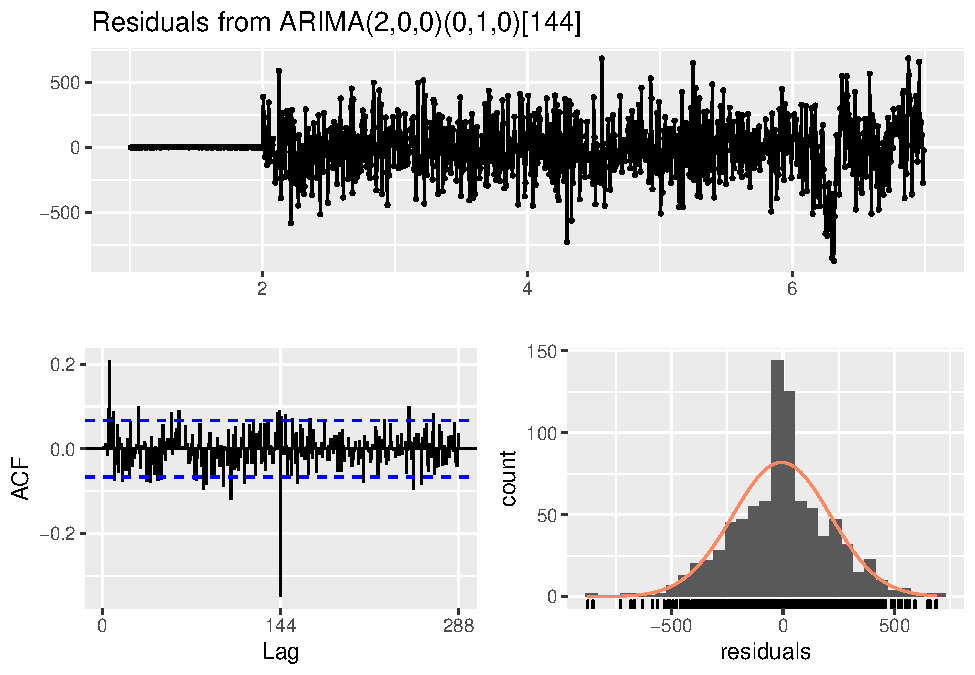
\includegraphics{document_files/figure-latex/unnamed-chunk-39-1.pdf}

\end{document}
